\chapter{Documentation}

\section{Compilation}
\label{sec:compilation}
La compilation d'un fichier \LaTeX{} nommé \og{}modele.tex\fg{} se fait au moyen des étapes suivantes (en lignes de commande)~:
%
\begin{itemize}
\item \verb+pdflatex modele+ (première compilation pour l'appel des différentes fonctionnalités contenues dans le mémoire)~;
\item \verb+bibtex modele+ (préparation de la bibliographie)~;
\item \verb+makeindex modele+ (préparation de l'index)~;
\item \verb+pdflatex modele+ (à faire 2 fois, produit le PDF complet).
\end{itemize}



%%%
% Images

\section{Les images}
\label{sec:images}

Le \index{Schéma} schéma~\ref{fig:schema} présente le schéma
d'annotation en entités nommées du domaine biomédical que nous avons
utilisé pour annoter nos corpus de données.
%
\begin{figure}[h]
  \centering
  %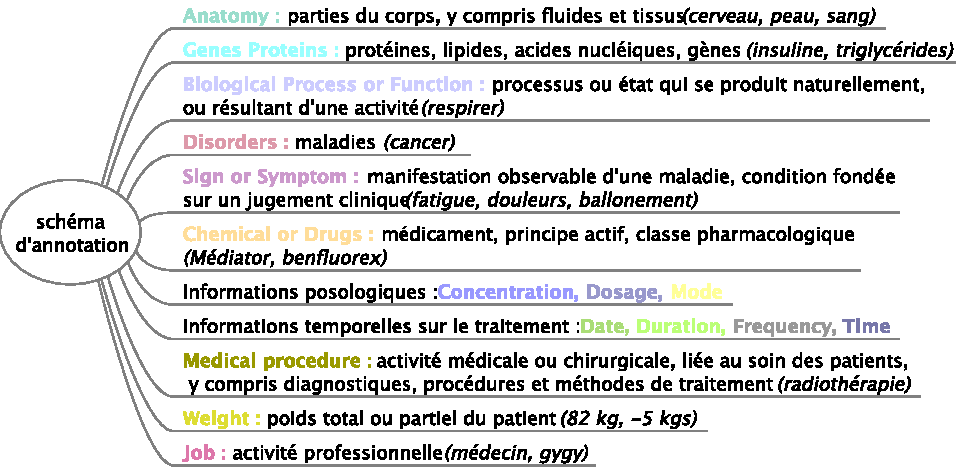
\includegraphics[width=.8\linewidth]{annotation2.pdf}
  \caption{Schéma d'annotation défini pour les entités nommées
    biomédicales}
  \label{fig:schema}
\end{figure}

L'intégration d'une image (format PDF, PNG) se fait au moyen de la
commande \verb+\includegraphics{fichier.pdf}+ avec d'éventuelles
options entre crochets pour spécifier la taille de l'image (height,
width) par rapport à la page.


%%%
% Tableaux

\newpage
\section{Les tableaux}
\label{sec:tableaux}

Pour réaliser un \index{Tableau} tableau en \LaTeX{}, la syntaxe
ressemble à (voir tableau~\ref{tab:exemple})~:
%
\begin{table}[h]
  \centering
  \begin{tabular}{|l|c|c|r|} \hline
    Expérience & Rappel & Précision & F-mesure \\ \hline
    Baseline & 0,372 & 0,500 & 0,427 \\
    Lexique & 0,907 & 0,903 & 0,905 \\
    Apprentissage & 0,880 & 0,942 & 0,910 \\ \hline
  \end{tabular}
  \caption{Résultats généraux pour chaque expérience}
  \label{tab:exemple}
\end{table}

Dans la commande \verb+\begin{tabular}{|l|c|c|r|}+ on définit le
  nombre de colonnes (ici 4), la manière dont le texte est mis en
  forme dans chaque colonne (l=left, c=center, r=right), et le
  séparateur de colonne (ici une ligne verticale). La commande
  \verb+\hline+ permet de tracer une ligne horizontale. La commande
  \verb+\caption{Titre ou légende}+ permet de définir la légende d'un
  tableau. Et la commande \verb+\label{nom}+ permet de nommer le
  tableau pour le désigner dans le corps du texte avec la commande
  \verb+\ref{nom}+ (e.g., tableau~\ref{tab:exemple}).

Les commandes \verb+\multirow{n}{*}{Texte}+ et
\verb+\multicolumn{n}{c}{Texte}+ permettent de fusionner plusieurs
lignes et plusieurs colonnes, avec $n$ le nombre de lignes ou colonnes
fusionnées. La commande \verb+\cline{2-4}+ permet de dessiner une
ligne horizontale de la colonne 2 à la colonne 4 (voir tableau~\ref{tab:autre}).
%
\begin{table}[h]
  \centering
  \begin{tabular}{|l|ccc|} \hline
    \multirow{2}{*}{Expérience} & \multicolumn{3}{c|}{Mesures} \\ \cline{2-4}
    & Rappel & Précision & F-mesure \\ \hline
    Baseline & 0,372 & 0,500 & 0,427 \\
    Lexique & 0,907 & 0,903 & 0,905 \\
    Apprentissage & 0,880 & 0,942 & \textbf{0,910} \\ \hline
  \end{tabular}
  \caption{Fusion de lignes et de colonnes dans un tableau}
  \label{tab:autre}
\end{table}


%%%
% Mise en forme

\section{Mise en forme}
\index{Mise en forme}
Il est possible de mettre du texte en \emph{emphase}
\verb+\emph{texte}+, en \textsl{version penchée}
\verb+\textsl{texte}+, en \textbf{gras} \verb+\textbf{texte}+, en
version \textsf{Sans Serif} (similaire à Arial et Helvetica)
\verb+\textsf{texte}+ ou encore en \textsc{Petites Capitales}
\verb+\textsc{Texte}+. Il n'est pas recommandé d'utiliser le
\underline{souligné} au vu de l'effet produit. Pour ajouter une note
de bas de page\footnote{Les notes de bas de page sont numérotées
  automatiquement en fonction de leur utilisation tout au long du
  texte. Avec ce modèle, la numérotation est remise à 1 à chaque début
  de chapitre.}, on utilise la commande
\verb+\footnote{Contenu}+. L'espace insécable (c.-à-d. qui ne peut pas
être coupée si elle est en fin de ligne), est représentée par le
tilde. On l'utilise généralement avant un appel de référence, ou avant
la référence d'un tableau ou d'une figure \verb+Tableau~\ref{clé}+.

Il est possible de ne pas numéroter les titres de section,
sous-section, etc., en utilisant la commande
\verb+\section{Titre}+. Dans ce cas, il est nécessaire d'ajuster les
mini tables des matières qui figurent au début de chaque chapitre au
moyen de la commande \verb+\adjustmtc+ en intégrant cette commande
autant de fois que nécessaire avant la commande \verb+\minitoc+

Pour forcer un saut de page, on utilise la commande \verb+\newpage+ et
pour un saut de ligne \verb+\\+


%%%
% Formules mathématiques

\section{Formules mathématiques}
\index{Rappel} Le rappel (formule~\ref{form:rappel}) mesure le nombre
d'éléments correctement étiquetés par le système (vrais positifs)
rapporté au nombre d'éléments étiquetés dans la référence (vrais
positifs et faux négatifs).
%
\begin{equation}
  \centering
  \text{Rappel} = {{\text{vrais positifs}}\over{\text{vrais positifs + faux négatifs}}}
  \label{form:rappel}
\end{equation}

\index{Precision@Précision} La précision
(formule~\ref{form:precision}) mesure le nombre d'éléments
correctement étiquetés par le système (vrais positifs) rapporté au
nombre total d'éléments étiquetés par le système (vrais et faux
positifs).
%
\begin{equation}
  \centering
  \text{Précision} = {{\text{vrais positifs}}\over{\text{vrais positifs + faux positifs}}}
  \label{form:precision}
\end{equation}

\index{F-mesure} La F-mesure (formule~\ref{form:fmesure}) est la
moyenne harmonique pondérée du rappel et de la précision. La valeur
accordée à $\beta$ permet de pondérer le rappel ou la précision, ou
d'équilibrer les deux mesures (avec $\beta=1$).
%
\begin{equation}
  \centering
  \text{F-mesure} = {{(1+\beta^2) \times \text{ précision } \times \text{ rappel }}\over{\beta^2 \times \text{ précision } + \text{ rappel } }}
  \label{form:fmesure}
\end{equation}

Les plus motivés d'entre vous pourront également réaliser des figures
(arbre syntaxique, histogramme, diagramme circulaire, etc.)
directement sous \LaTeX{} en utilisant le package Tikz\footnote{Voir
  \url{http://bertrandmasson.free.fr/index.php?categorie6/latex-pgf-tikz}
  pour de nombreux exemples utiles.} une fois qu'ils auront terminé la
rédaction de leur mémoire pour ne pas perdre de temps dès le départ...


%%%
% Bibliographie

\section{Gestion de la bibliographie}
La \index{Bibliographie} bibliographie figure dans un fichier nommé
\og{}biblio.bib\fg{}. Ce fichier peut être édité dans un éditeur de
texte classique \emph{(emacs, vi, notepad)}, ou par le biais d'un
outil de gestion de bibliographie tel que \textsf{JabRef}, un
programme Java qui permet de gérer efficacement les fichiers *.bib et
de remplir les différents champs nécessaires à chaque entrée.

\subsection{Appels de référence}
On appelle les références au moyen de la
commande \verb+\cite{clé}+ avec une clé de citation qui est définie
dans la bibliographie. On intègre généralement une référence
bibliographique après avoir introduit le concept. Par exemple~: nos
expériences en approche statistique reposent sur le formalisme des
CRF~\cite{lafferty-2001icml} implémenté dans l'outil
WAPITI~\cite{lavergne-2010acl}. Nous avons suivi le protocole défini
par~\cite[p.~3]{grouin-2014jbi} pour constituer les annotations de corpus.

Il est possible de citer plusieurs articles en même temps en séparant
chaque clé par une virgule. Par exemple~: notre travail repose sur la
détection d'entités nommées~\cite{ehrmann2008phd, sekine-2009} du
domaine biomédical, en particulier la détection des mentions de
bactéries et de biotopes~\cite{bossy-2012bb}.


\subsection{Format}
\LaTeX{} gère automatiquement le format de présentation des
références, selon que l'article cité a été rédigé par un
auteur~\cite{ehrmann2008phd} (auquel cas sont mentionnés le nom et
l'année), deux auteurs~\cite{bretonnel-2008plos} (les noms des deux
auteurs et l'année), ou plus de deux auteurs~\cite{brown-1992cl} (le
nom du premier auteur, la mention \emph{et al.}\footnote{Locution
  latine signifiant \og{}et d'autres\fg{}.}, et l'année).

